\documentclass[a4paper, UKenglish]{article}
%% Encoding
\usepackage[utf8]{inputenx}
\usepackage[T1]{fontenc}

%% Fonts and typography
\usepackage{lmodern}           % Latin Modern Roman
\usepackage[scaled]{beramono}  % Bera Mono (Bitstream Vera Sans Mono)
\renewcommand{\sfdefault}{phv} % Helvetica
\usepackage[bf, sf]{titlesec}  % Section headings
\usepackage[final]{microtype}  % Improved typography


%% Mathematics
\usepackage{amssymb}   % Extra symbols
\usepackage{amsthm}    % Theorem-like environments
\usepackage{thmtools}  % Theorem-like environments
\usepackage{mathtools} % Fonts and environments for mathematical formuale
\usepackage{mathrsfs}  % Script font with \mathscr{}
\usepackage{amsmath}


%% Miscellanous
\usepackage{graphicx}   	% Tool for images
\usepackage{subcaption} 	% Tool for images
\usepackage[UKenglish]{babel}   % Automatic translations
\usepackage{csquotes}   	% Quotes
\usepackage{textcomp}   	% Extra symbols
\usepackage{booktabs}   	% Tool for tables
\usepackage{float}

\usepackage[usenames,dvipsnames]{xcolor}
\definecolor{lbcolor}{rgb}{0.9,0.9,0.9}
\usepackage{listings}   % Typesetting code
%\lstset{backgroundcolor=\color{lbcolor}, basicstyle = \ttfamily, frame = %single, language=python}
\lstset{
	backgroundcolor=\color{lbcolor},
	tabsize=4,
	rulecolor=,
	language=java,
        basicstyle=\scriptsize,
        upquote=true,
        aboveskip={1.5\baselineskip},
        columns=fixed,
	numbers=left,
        showstringspaces=false,
        extendedchars=true,
        breaklines=true,
        prebreak = \raisebox{0ex}[0ex][0ex]{\ensuremath{\hookleftarrow}},
        frame=single,
        showtabs=false,
        showspaces=false,
        showstringspaces=false,
        identifierstyle=\ttfamily,
        keywordstyle=\color[rgb]{0,0,1},
        commentstyle=\color[rgb]{0.133,0.545,0.133},
        stringstyle=\color[rgb]{0.627,0.126,0.941}
        }

%% Bibliography
\usepackage[backend = biber, style = alphabetic]{biblatex}
%\addbibresource{<NAME OF BIBLIOGRAPY FILE>.bib}


%% Cross references
\usepackage{varioref}
\usepackage{hyperref}
\urlstyle{sf}
\usepackage[nameinlink, capitalize, noabbrev]{cleveref}


%% Theorem-like environments
\declaretheorem[style = plain, numberwithin = section]{theorem}
\declaretheorem[style = plain,      sibling = theorem]{corollary}
\declaretheorem[style = plain,      sibling = theorem]{lemma}
\declaretheorem[style = plain,      sibling = theorem]{proposition}
\declaretheorem[style = definition, sibling = theorem]{definition}
\declaretheorem[style = definition, sibling = theorem]{example}
\declaretheorem[style = remark,    numbered = no]{remark}


%% Delimiters
\DeclarePairedDelimiter{\p}{\lparen}{\rparen}   % Parenthesis
\DeclarePairedDelimiter{\set}{\lbrace}{\rbrace} % Set
\DeclarePairedDelimiter{\abs}{\lvert}{\rvert}   % Absolute value
\DeclarePairedDelimiter{\norm}{\lVert}{\rVert}  % Norm


%% Operators
\DeclareMathOperator{\im}{im}
\DeclareMathOperator{\rank}{rank}
\DeclareMathOperator{\E}{E}
\DeclareMathOperator{\Var}{Var}
\DeclareMathOperator{\Cov}{Cov}


%% New commands for sets
\newcommand{\N}{\mathbb{N}}   % Natural numbers
\newcommand{\Z}{\mathbb{Z}}   % Integers
\newcommand{\Q}{\mathbb{Q}}   % Rational numbers
\newcommand{\R}{\mathbb{R}}   % Real numbers
\newcommand{\C}{\mathbb{C}}   % Complex numbers
\newcommand{\A}{\mathbb{A}}   % Affine space
\renewcommand{\P}{\mathbb{P}} % Projective space


%% New commands for vectors
\renewcommand{\a}{\mathbf{a}}
\renewcommand{\b}{\mathbf{b}}
\renewcommand{\c}{\mathbf{c}}
\renewcommand{\v}{\mathbf{v}}
\newcommand{\w}{\mathbf{w}}
\newcommand{\x}{\mathbf{x}}
\newcommand{\y}{\mathbf{y}}
\newcommand{\z}{\mathbf{z}}
\newcommand{\0}{\mathbf{0}}
\newcommand{\1}{\mathbf{1}}


%% Miscellanous
\renewcommand{\qedsymbol}{\(\blacksquare\)}


%% Things I've put in meself
\usepackage{tikz}
\usetikzlibrary{decorations.pathreplacing,angles,quotes}
\newcommand*\circled[1]{\tikz[baseline=(char.base)]{
            \node[shape=circle,draw,inner sep=2pt] (char) {#1};}}
\usepackage{arydshln}



\begin{document}
\title{FYS-STK 3155 project 1}
\author{Theodor Midtbø Alstad}
\maketitle

\begin{abstract}
The project detailed in this report is unfinished due to time constraints, and has many ways it could be improved.

This project aims to explore linear regression, with the final goal of learning and predicting the geography of an area. The project is split into 7 sections, labelled a) through g), culminating in application to geographical data in section g), and will be referred to as such in the report. 

The final goal of fitting models to geographical data is not met, and the best fit gotten is a model with an $R^2$ score of -125.


\end{abstract}

\section{Introduction}
This project implements the regression methods Ordinary Least Squares, LASSO, and Ridge, with the resampling methods bootstrap and k-fold cross-validation.

The project starts by modelling the Franke function in the for the domain $x,y \in [0,1]$, before moving on to geographical data at the end.

Throughout the project, multiple bias-variance and test-train MSE analyses are done, combining the regression- and resampling methods to do so. 

The goal of this project is two-fold; to model geographical data and to learn more about, and evaluate, the regression methods implemented.
  
  
\subsection{The structure of the source code}
The code is written in python3, formatted as a cascading inheriting class structure. That is, section b) inherits from the class of section a), section c) inherits from the class of section b), and so on.

All outputs are found in the outputs folder, as detailed in the .README file.

\subsection{Franke function} \label{sec:Franke}
The Franke function is modelled in sections a) through e), as a placeholder for geographical data in section g). It is here defined for the domain $x,y \in [0,1]$
\begin{align*}
f(x,y) &= \frac{3}{4}\exp{\left(-\frac{(9x-2)^2}{4} - \frac{(9y-2)^2}{4}\right)}+\frac{3}{4}\exp{\left(-\frac{(9x+1)^2}{49}- \frac{(9y+1)}{10}\right)} \\
&+\frac{1}{2}\exp{\left(-\frac{(9x-7)^2}{4} - \frac{(9y-3)^2}{4}\right)} -\frac{1}{5}\exp{\left(-(9x-4)^2 - (9y-7)^2\right) }
\end{align*}

\subsection{Ordinary Least Squares (OLS)}
The OLS method attempts to model a dataset by minimizing the square error between the dataset, $y$, and a model in the form of $\hat{y} = \textbf{X} \beta$, where $\textbf{X}$ is a design matrix and $\beta$ is a vector of parameters.

OLS successfully and analytically minimizes the cost function $C = \mathbb{E}[(y - \hat{y})^2]$ by using parameters $$\beta = \left(\textbf{X}^T\textbf{X}\right)^{-1} \textbf{X}^T y $$

\subsection{Bias \& Variance}
Using a cost function $C$ based on the Mean Square Error between our prediction, $\hat{y}$, and the recorded value, $y = f(x) + \epsilon$, the bias and variance can be found as

\begin{align*}
(y - \hat{y})^2 &= (y + (\mathbb{E}[\hat{y}] - \mathbb{E}[\hat{y}]) -\hat{y})^2
\\&= ((y + \mathbb{E}[\hat{y}]) - (\mathbb{E}[\hat{y}] -\hat{y}))^2
\\&= (y- \mathbb{E}[\hat{y}])^2 + (\mathbb{E}[\hat{y}] - \hat{y}) \\&+ 2(y - \mathbb{E}[\hat{y}])(\mathbb{E}[\hat{y}] - \hat{y})
\\\\
C &= \mathbb{E}[(y - \hat{y})^2]
\\&= \mathbb{E}[(y- \mathbb{E}[\hat{y}])^2 + (\mathbb{E}[\hat{y}] - \hat{y}) \\&+ 2(y - \mathbb{E}[\hat{y}])(\mathbb{E}[\hat{y}] - \hat{y})]
\\&= \mathbb{E}[(y- \mathbb{E}[\hat{y}])^2] + \mathbb{E}[(\mathbb{E}[\hat{y}] - \hat{y})] \\&+ \mathbb{E}[2(y - \mathbb{E}[\hat{y}])(\mathbb{E}[\hat{y}] - \hat{y})]
\\\\
\mathbb{E}[2(y - \mathbb{E}[\hat{y}])(\mathbb{E}[\hat{y}] - \hat{y})]&=2(y - \mathbb{E}[\hat{y}])\mathbb{E}[(\mathbb{E}[\hat{y}] - \hat{y})]
\\&= 2(y - \mathbb{E}[\hat{y}])\times 0
\\&=0
\\\\
\mathbb{E}[(y- \mathbb{E}[\hat{y}])^2] &= \mathbb{E}[((f(x) + \epsilon) - \mathbb{E}[\hat{y}])^2]
\\&= \mathbb{E}[((f(x) - \mathbb{E}[\hat{y}]) + \epsilon)^2]
\\&= \mathbb{E}[(f(x) - \mathbb{E}[\hat{y}])^2 + \epsilon(f(x) -\mathbb{E}[\hat{y}]) + \epsilon^2]
\\&= \mathbb{E}[(f(x) - \mathbb{E}[\hat{y}])^2 + 0 + \epsilon^2]
\\&= \mathbb{E}[(f(x) - \mathbb{E}[\hat{y}])^2] + \mathbb{E}[\epsilon^2]
\\&= \mathbb{E}[(f(x) - \mathbb{E}[\hat{y}])^2] + \sigma^2
\\\\
C &= \mathbb{E}[(f(x) - \mathbb{E}[\hat{y}])^2] + \mathbb{E}[(\mathbb{E}[\hat{y}] - \hat{y})] + \sigma^2
\end{align*}

where $\mathbb{E}[(f(x) - \mathbb{E}[\hat{y}])^2]$ is the bias, $\mathbb{E}[(\mathbb{E}[\hat{y}] - \hat{y})]$ is the variance, and $\sigma^2$ is the irreducible error.\\
Bias can be interpreted as the expected mean square error between a prediction and their true values, and is often used to determine how well fitted a model is. It usually goes down with the complexity of a model, as the model is more able to bend to the training points.\\
Variance can be interpreted as how much a model varies over multiple iterations, and is often used to determine whether a model is overfitted to its test data. It usually goes up with the complexity of a model, as the model will twist, bend, and turn more to fit the training points.\\
The irreducible error is an error that cannot be overcome by improving the model, and can be attributed to things such as noise.

\subsection{Bootstrap Resampling}
The bootstrap resampling method aims to evaluate a regression method by generating multiple training sets to a single test set. It accomplishes this by initially splitting a complete data set into training and test sets, then repeatedly creating \textit{sample} sets by picking out random points from the training set (duplicates are allowed in the sample set) until the sample set has a set size (in this report sample sets are given 80\% size of the initial training set). Then the regression model is applied to the sample set, evaluated against the testing set, another sample set is drawn, and this is repeated as many times as is specified. An average calculated per evaluation method, and used as an estimate for the evaluation of the regression method.

\subsection{K-fold cross-validation resampling}
Another resampling method, and the last that will be used here, k-fold cross-validation splits a dataset into k equally sized sets, and treats one of them at a time as a testing set while treating the collection of the remaining $k-1$ sets collectively as a training set. Any evaluations using k-fold cross-validation are evaluated as an average over the k test sets.

\subsection{Ridge}
The ridge method is an adjustment to the OLS method, and involves introducing a term that is added to the matrix about to be inverted, in the form of a scalar constant $\lambda$ multiplied into an identity matrix. This helps makes uninvertible matrices invertible, and assists the models accuracy. 
$$\beta = \left(\textbf{X}^T\textbf{X} + \lambda \textbf{I}\right)^{-1} \textbf{X}^T y $$
They key to using Ridge is finding an optimal $\lambda$.

\subsection{Lasso}
The lasso method differs slightly from ridge in that it attempts to minimize $\displaystyle\sum_{n}^{i=1} \left( y_i - \beta_0 - x_i^T\beta  \right)^2$ in terms of $\beta$. In this report, scikit learn's method is used in place of creating one; 

\begin{lstlisting}[language=Python]
# Python example of lasso implementation using the sklearn module
# Assuming dataset has been split into X_train, X_test, y_train, and y_test

import sklearn.linear_model as linmod
lassoAlpha = 0.1
clf = linmod.Lasso(alpha=lassoAlpha)
clf.fit(X_train, y_train)
ypredict = clf.predict(X_test)
\end{lstlisting}

\section{Method}
\subsection{Data generation} \label{sec: dataGen}
The class is given 3 initial arguments; n, p, and noisefactor. n refers to the square of the number of data points used, p refers to the polynomial degree of the design matrix, and noisefactor refers to the amount of noise that should be present in the data.

Raw data generation:
\\First, $\frac{n}{2}$ points, rounded up, are distributed with linear distribution within the domain of Franke; between 0 and 1. 
\\Second, $\frac{n}{2}$ points, rounded down, are distributed with uniform random distribution within the same domain. 
\\Third, these two sets are combined to form a 1D dataset. 
\\Fourth, this is repeated and the two datasets, x and y, are made to form a meshgrid which is then flattened, creating an even and reliable full, 2D dataset. It is noted that this is a better dataset than one could expect normally, but a similar method is used to extract data from the geographical dataset when the required space or processing power  for the full dataset is not available. 
\\Fifth, expected data is generated  from these data with the Franke function. 
\\Sixth, normally distributed noise of mean 0 and variance 1, multiplied by the noise factor and the mean of the Franke data, are added to the Franke data.

\begin{lstlisting}[language=Python]
def __init__(self, n, p, noisefactor = 0.1):
  x1 = y1 = np.linspace(0, 1, mt.ceil(n/2))
  x2 = np.random.uniform(0, 1, mt.floor(n/2))
  y2 = np.random.uniform(0, 1, mt.floor(n/2))
  
  x = np.concatenate((x1, x2))
  y = np.concatenate((y1, y2))
  
  x, y = np.meshgrid(x,y)
  self.x = x.flatten()
  self.y = y.flatten()
  
  self.ytrue = self.FrankeFunction(self.x, self.y)
  self.yData = self.ytrue + noisefactor*np.random.randn(n**2)*self.ytrue.mean()
\end{lstlisting}

Design Matrix generation:
The design matrix is made as a polynomial set of x and y, where each column is a polynomial product of the two, and the rows are points of data. The non-constant columns (i.e. all columns but the first) are scaled by subtracting the average value of each respective column from itself.

\begin{lstlisting}[language=python]
def craftX(self, scaling=True):
  self.nfeatures = int(((self.p+1)*(self.p+2))/2)
  self.X = np.zeros((len(self.x), self.nfeatures))

  ind = 0
  for i in range(self.p+1):
    for j in range(self.p+1-i):
      self.X[:,ind] = self.x**i * self.y**j
      ind += 1

  if scaling:
    self.X[:,1:] -= np.mean(self.X[:,1:], axis=0)
\end{lstlisting}

\subsection{a) Ordinary Least Square (OLS) on the Franke function}
Implemented in this section:
\begin{itemize}
\item Data generation
\item $R^2$ score function
\item Mean Squared error (MSE) evaluation function
\item Design Matrix \& Franke values
\item OLS
\item Method to find the 95\% confidence intervals of the beta parameters of the OLS-method
\end{itemize}

\begin{lstlisting}[language=python]
# Main OLS method
beta = np.linalg.pinv(X_train.T @ X_train) @ X_train.T @ y_train
\end{lstlisting}

\begin{lstlisting}[language=python]
def MSE(self, y_data, y_model):
    # Optimal value is 0, with higher values beign worse
    return np.sum((y_data-y_model)**2) / np.size(y_model)

def R2(self, y_data, y_model):
    # Optimal value is 1, with 0 implying that model performs 
    # exactly as well as predicting using the data average would.
    # Lower values imply that predicting using the average would be better
    top = np.sum((y_data - y_model)**2)
    bot = np.sum((y_data - np.mean(y_data))**2)
    return 1 - top/bot
\end{lstlisting}

This section generated data as described in \cref{sec: dataGen}, attempted to model it with an OLS approximation, and evaluated the MSE, $R^2$ score, and the confidence interval of the $\beta$-parameters.

The confidence interval of the $\beta$-parameters was found by running an OLS model 300 times, finding 300 examples of the $\beta$-parameters, calculating the standard deviation, $\sigma$, for the parameters, then adding and subtracting $1.645\sigma$ to and from the mean of the parameters.

\subsection{b)Bias-variance trade-off and resampling techniques} \label{sec:method b)}
Implemented in this section:
\begin{itemize}
\item OLS plotting training and test MSE's over complexity
\item OLS with bootstrap resampling technique
\item Bias-variance analysis
\end{itemize}

This section aimed to evaluate OLS by plotting error in testing and training data together against a varying complexity in the model, evaluate OLS by using bootstrap resampling, and perform a bias-variance trade-off analysis using bootstrap.

Noisefactor is set to 0 in this section to find an error in the calculations for bias and variance.

\begin{lstlisting}[language=python]
def sample(self, sourceX, sourceY, Nsamples = 0.6):
    if isinstance(Nsamples, float):
        Nsamples = int(Nsamples*sourceX.shape[0])

    sampleArrayX = np.zeros(sourceX[:Nsamples,:].shape)
    sampleArrayY = np.zeros(Nsamples)
    for i in range(Nsamples):
        ind = np.random.randint(Nsamples)
        sampleArrayX[i] = sourceX[ind]
        sampleArrayY[i] = sourceY[ind]

    return sampleArrayX, sampleArrayY
\end{lstlisting}

\begin{lstlisting}[language=python]
def bootstrap(self, sampleSize=None, sampleN=None):
    if sampleSize is None: sampleSize = 0.8
    if sampleN is None: sampleN = 5
    self.craftX()
    if isinstance(sampleSize, float): sampleSize = int(sampleSize*len(self.x))
    r2list, SElist = np.zeros((2, sampleN)) 
    X_train, X_test, y_train, y_test = train_test_split(self.X, self.yData)
    for i in range(sampleN):
        X_sample, y_sample = self.sample(X_train, y_train)
        r2list[i], SElist[i] = self.OLS([X_sample, X_test, y_sample, y_test])[:2]
    return r2list, SElist
\end{lstlisting}

\begin{lstlisting}[language=python]
def bias(self, y_data, y_model):
    return np.mean((y_data - np.mean(y_model, axis=1))**2)
    
def variance(self, y_model):
    return np.mean(np.var(y_model, axis=1))
\end{lstlisting}

The bias-variance analysis was implemented by using bootstrap OLS over a range of polynomial complexities and plotting the bias, variance, and the MSE. It similarly plotted the training MSE and test MSE over complexity.

\subsection{c) Cross-validation as resampling techniques, adding more complexity}
Implemented in this section: 
\begin{itemize}
\item k-fold cross-validation
\end{itemize}

This section implements k-fold cross-validation resampling and compares it to bootstrap resampling, using the same evaluation methods of $R^2$ and MSE. k-fold cross-validation and bootstrap are compared for equivalent number of folds and number of samples, 5 and 10.

The k-fold crossvalidation was implemented in three functions; kfold\_splitter(), kfold\_yielder(), and kfold(). kfold\_splitter() shuffles and splits the data into several versions of training sets and testing sets, as a 3D-array for the inputs and a 2D-array for the outputs, functioning as collections of 2D-arrays and 1D-arrays. kfold\_yielder() then functions as a generator, supplying these sets as appropriate 2- and 1D-arrays to kfold(), which performs OLS on the sets generated in turn.

\subsection{d) Ridge Regression on the Franke function with resampling}
Implemented in this section: 
\begin{itemize}
\item Ridge
\item Ridge with bootstrap
\item Ridge with k-fold cross-validation
\end{itemize}

This section implements Ridge and applies bootstrap and k-fold cross-validation resampling techniques to it. It was also supposed to implement a bias-variance analysis, but as of this moment, it is only a copy of the function defined in partB.py, and does not do the job it's supposed to.

\subsection{e) Lasso Regression on the Franke function with resampling}
Implemented in this section: 
\begin{itemize}
\item Lasso method
\item Bias-variance analysis using lasso and bootstrap
\end{itemize}


This section implements scikit learn's lasso method with no resampling and inserts it into a bias-variance analysis function with bootstrap resampling, similar to what was done in \autoref{sec:method b)}.

\begin{lstlisting}[language=python]
def lasso(self, alpha=None):
    if alpha is None: alpha = 5
    clf = linmod.Lasso(alpha=alpha)
    self.craftX()
    X_train, X_test, y_train, y_test = train_test_split(self.X, self.yData)
    clf.fit(X_train, y_train)
    ypredict = clf.predict(X_test)
    return self.R2(y_test, ypredict), self.MSE(y_test, ypredict)
\end{lstlisting}

\subsection{f) Introducing real data and preparing the data analysis}
Implemented in this section:
\begin{itemize}
\item Geographical data
\end{itemize}

This section imports geographical data from [1]

\begin{figure}[H]
        \centering 
        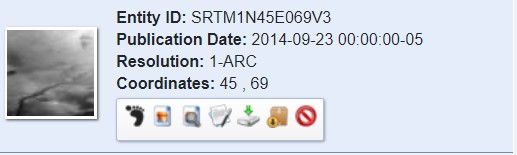
\includegraphics[scale=0.75]{../Source_code/geodata/SRTM1N45E069V3.jpg} 
        \caption{Metadata for the data downloaded.}
        \label{fig:geodata metadata}
\end{figure}

\subsection{g) OLS, Ridge and Lasso regression with resampling}
Implemented in this section:
\begin{itemize}
\item New data generation
\end{itemize}

This section was intended to use all methods developed previously on the geographical data, compared and evaluated them against each other as viable methods. The ridge method was to be prepared as a 2D heatmap of polynomial complexity and $\lambda$-value. The methods were to be compared to scikit learn's methods to evaluate them as relatively simple implementations against more complex ones. Given the time constraints, the majority of this has not been implemented. 

This section, instead, implements geographical data extraction and the train-test MSE over polynomial complexity from section b) over this dataset.

There also exists in the code an unfinished k-fold cross-validation version of the this train-test plot, but this was not completed in time.






\section{Results/Discussion}
Results (printouts) are described in more detail for each section in the folder outputs/.
\subsection{a) Ordinary Least Square (OLS) on the Franke function}
With 10,000 datapoints and a polynomial degree of 5, OLS reaches an $R^2$ value of 0.95 with an MSE of 0.004. If the data generation method is changed to being $n^2$ points linearly distributed between (0,0), (0,1), (1,0) and (1,1), the $R^2$ rises to 0.96, indicating that the extra steps taken to vary the dataset actually hinders the quality of the model.


\subsection{b) Bias-variance trade-off and resampling techniques}
\begin{figure}[H]
        \centering 
        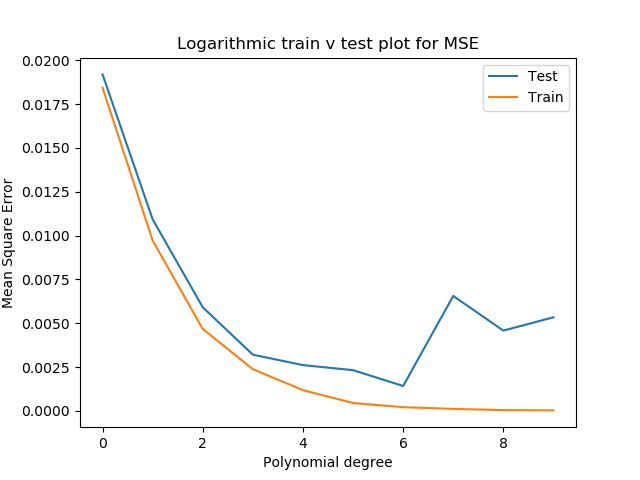
\includegraphics[scale=0.75]{../outputs/images/partB/trainTestMSE.png} 
        \caption{Testing and training errors proceeding as expected over model complexity; training error is continually falling whilst testing data falls to a point and then rises again due to overfitting.}
        \label{fig:trainTestMSE}
\end{figure}
\begin{figure}[H]
        \centering 
        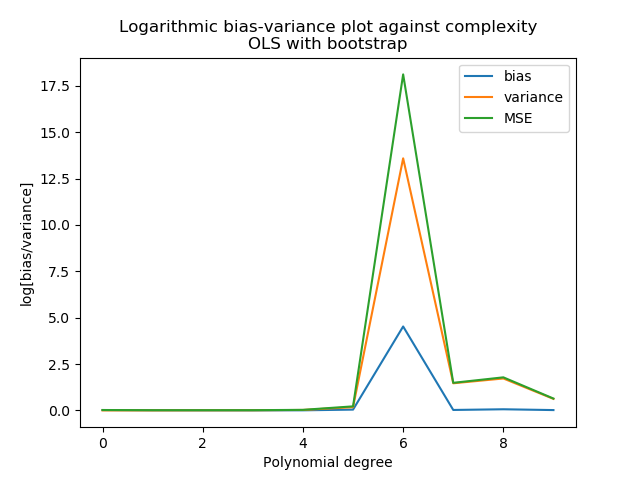
\includegraphics[scale=0.75]{../outputs/images/partB/biasVariance.png} 
        \caption{Bias and variance behaving unextpectedly, having a massive spike 17 orders of magnitude above the rest in both bias and variance.}
        \label{fig:biasVariance}
\end{figure}

\autoref{fig:biasVariance} suggests that something has gone wrong during the calculations of bias and variance. Possible reason include:
\begin{itemize}
\item A poor model: In addition to the well-behaved \autoref{fig:trainTestMSE}, my model has been compared to sklearns model (see lines 101-104 of partB.py) and both models exhibit this behaviour.
\item Incorrect equations for bias, variance or MSE: All three values are calculated independently, and the relationship MSE = Bias + Variance is found consistently (see last line of printout in outputs/partB.txt or line 114 in partB.py), implying that the calculations are correct.
\end{itemize}
I have been unable to find any other source of error in the time I have for this project.


\subsection{c) Cross-validation as resampling techniques, adding more complexity}

\begin{lstlisting}[language=python]
Folds/number of samples:  5
k-fold          [R2, MSE] : [0.95563823 0.00368468]
Bootstrap       [R2, MSE] : [0.9545114  0.00377724]
kfold/bootstrap [R2, MSE] : [1.00118054 0.9754959 ]

Folds/number of samples:  10
k-fold          [R2, MSE] : [0.95312732 0.00396122]
Bootstrap       [R2, MSE] : [0.9526719  0.00386939]
kfold/bootstrap [R2, MSE] : [1.00047805 1.02373248]
\end{lstlisting}

Comparing 5-fold cross-validation against 5-sample bootstrap and 10-fold cross-validation against 10-sample bootstrap shows that the $R^2$ and MSE values are very similar, suggesting that the reasmpling methods have no impact on the actual accuracy of the model. 

\subsection{d) Ridge Regression on the Franke function with resampling}
\begin{lstlisting}[language=python]
Normal OLS; average values:
OLS, multiple times [R2, MSE] : [0.9533851 0.0038293]
Bootstrap           [R2, MSE] : [0.9545558 0.0038718]
kfold               [R2, MSE] : [0.9540727 0.0037702]

Ridge application; optimal values:
Bootstrap       [R2, MSE] : [0.9524293 0.0039346]
k-fold          [R2, MSE] : [0.9540655 0.0037696]
\end{lstlisting}

The optimal value for $\lambda$ is $\lambda = 0$, meaning that for this application, ridge provides no benefit, but it also does not detract from the accuracy in any substantial way.

\begin{figure}[H]
        \centering 
        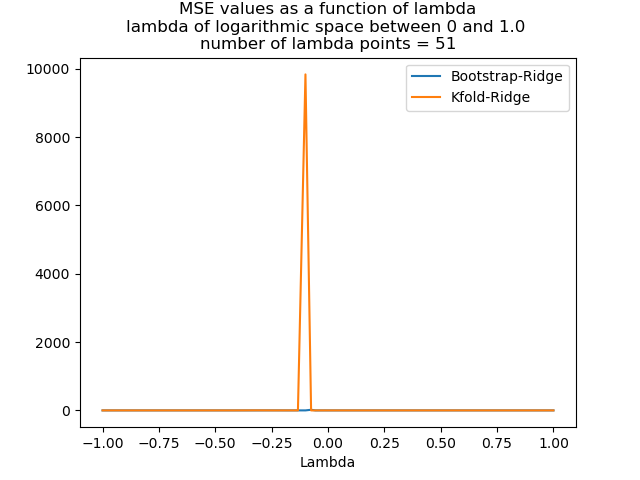
\includegraphics[scale=0.75]{../outputs/images/partD/MSERidge.png} 
        \caption{Ridge implemented a variable for MSE, using both bootstrap and k-fold cross-validation resampling methods. There is a big spike on the negative side of 0, possibly implying that the matrix is not invertible in that area, or that the issue seen in \autoref{fig:biasVariance} may extend to this.}
        \label{fig:MSERidge}
\end{figure}
\begin{figure}[H]
        \centering 
        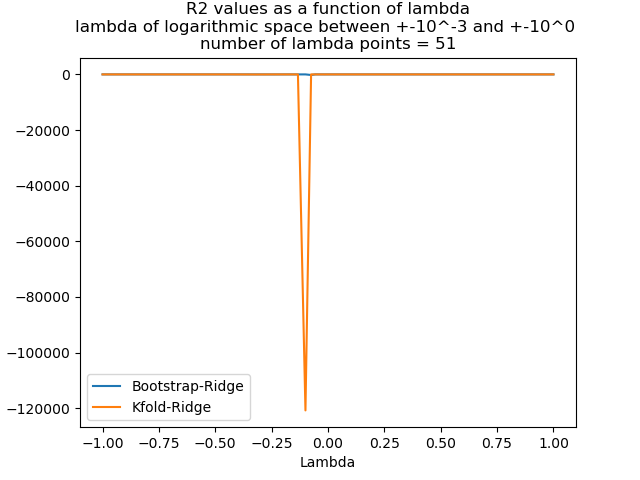
\includegraphics[scale=0.75]{../outputs/images/partD/R2Ridge.png} 
        \caption{Similar to \autoref{fig:MSERidge}, this figure presents the $R^2$-evaluation, seeing a big dip on the negative side of 0.}
        \label{fig:R2Ridge}
\end{figure}


\subsection{e) Lasso Regression on the Franke function with resampling} \label{sec:results Lasso}
\begin{lstlisting}[language=python]
Lasso evaluation [R2, MSE] at alpha = 0.01: 
  (-0.00040418848759649073, 0.09415771032493848)
Lasso evaluation [R2, MSE] at alpha =  0.1: 
  (-0.0008014043714434926, 0.09901736017684995)
Lasso evaluation [R2, MSE] at alpha =  0.3: 
  (-6.013665053505868e-05, 0.09889216375005189)
Lasso evaluation [R2, MSE] at alpha =    1: 
  (-0.00011187832184433866, 0.09252839549202323)
Lasso evaluation [R2, MSE] at alpha =    3: 
  (-0.00013499053518417625, 0.09445379258455494)
MSE/(bias+variance) = [1. 1. 1. 1. 1. 1. 1. 1. 1. 1.]
\end{lstlisting}


The lasso implementation reaches an $R^2$ value of -0.001, which is a very poor value, but it also reaches an MSE value down to 0.08, implying that the model might not be bad, but that something else could have gone wrong. This may be a similar issue to what occurs in \autoref{fig:biasVariance}


\begin{figure}[H]
        \centering 
        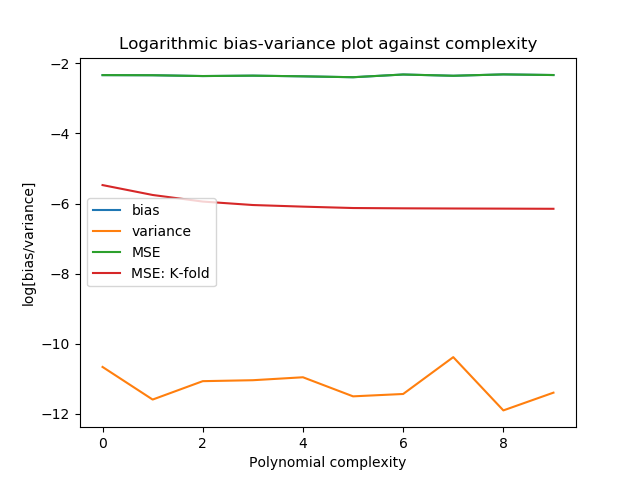
\includegraphics[scale=0.75]{../outputs/images/partE/lassoBiasVariance.png} 
        \caption{Bias is hidden by the MSE. MSE:K-fold is the MSE calculated during the caluculations, rather than after-the-fact, and the two MSE's disagree, implying that something has gone wrong.}
        \label{fig:LassoBiasVariance}
\end{figure}

\subsection{f) Introducing real data and preparing the data analysis}
\begin{figure}[H]
        \centering 
        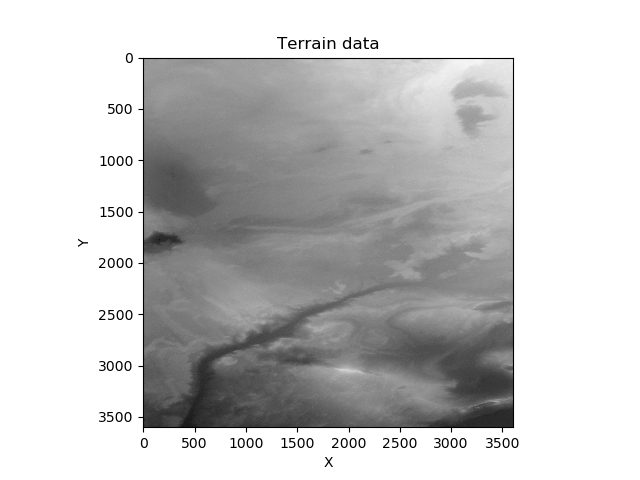
\includegraphics[scale=0.75]{../Source_code/geodata/geodata_area.png} 
        \caption{Geographical data, represented on a gray scale.}
        \label{fig:geodata}
\end{figure}

\subsection{g) OLS, Ridge and Lasso regression with resampling}

\begin{figure}[H]
        \centering 
        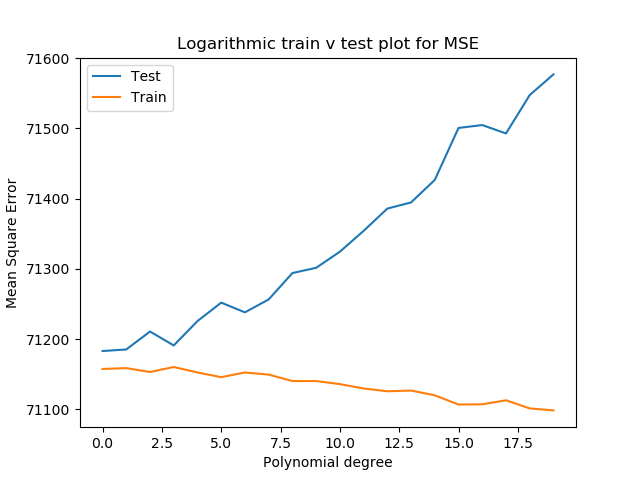
\includegraphics[scale=0.75]{../outputs/images/partG/trainTestMSE.png} 
        \caption{}
        \label{fig:geodata}
\end{figure}

\begin{lstlisting}
R2: ( avg = -126.007750214505 )
    ( max = -125.28996659328048 )
    ( min = -126.63064184509612 )
 [-125.28996659 -126.00075666 -125.99061752 
  -126.63064185 -126.33000825 -125.80451042]

MSE: ( avg = 71177.81149110844 )
     ( max =  71218.32821713865 )
     ( min =  71113.55185997034 )
 [71175.41435112 71218.32821714 71167.27618466 
  71178.49262646 71213.80570729 71113.55185997]
\end{lstlisting}

Given the lack of different evaluations, it is difficult to see anything in the data; the poor values could be due to OLS being a poor fit for this data, or it could be a poor implementation. Without additional approaches or different real datasets to compare to, it is difficult to say.


\section{Conclusion}
This project is riddled with symptoms of being unfinished, and there are few conclusions to be drawn. There are, however, many things to improve on. The initial train-test plot in section b) seems promising, indicating that the base Franke data generation, the basic OLS implementation, and the base evaluation methods are all implemented properly, and fit well with the data. I don't currently have enough information to be able to tell what is wrong with the bias-variance plot in the same section, but given how early it is implemented (although chronologically it was implemented near the end of the project) it should be one of the first places that are looked to for errors and mistakes.

The large spike in the ridge plots in section d) implies that there might be an issue regarding the invertibility of $\textbf{X}^T\textbf{X}$, which might lead to very unstable solutions near $\lambda = 0$, which includes the general OLS-solution. This can serve as part of a one-of-many-problems explanation, but is unlikely to be the entire issue, given that the train-test plot and bias-variance plots in section b) behave so differently.

Section c) shows that the resampling methods, bootstrap and k-fold cross-validation, seem to behave well, indicating that they are well implemented and function well for the Franke dataset. Although their aptness for the dataset is derived purely from the base model they use in this instance, OLS, and from the resampling methods themselves, so their fitting the Franke dataset is no surprise given that OLS already fit.

The Lasso implementation, as mentioned in \autoref{sec:results Lasso}, has a curious case of a consistently poor $R^2$ and a consistently good MSE. This is made even more curious by the fact that this is scikit learn's own method implemented, and that it predicts with similar accuracy to a straight average ($R^2$ score of near 0). Unfortunately, there has not been enough time to look into this curiousity.

The only conclusion that could be drawn about the final section, section g), is that the model used to model it is a poor fit at all complexities used, unfortunately. This section could benefit most from more time, even though I believe that time would have to start at the beginning and root out errors that may propagate throughout the entire project.

Finally, the entire source code needs to have bugs rooted out, functions commented, a greater generalization, a refactoring, and to be finished. Unfortunately, I cannot do this given that I don't have the time to.


\section{References}
\begin{itemize}
\item [1] https://earthexplorer.usgs.gov/
\item [2] Trevor Hastie, Robert Tibshirani, and Jerome Friedman. \textit{The Elements of Statistical Learning}. Springer, 2017
\end{itemize}


\newpage
\section{Appendix}
\subsection{Source code}
\subsubsection{a) Ordinary Least Square (OLS) on the Franke function}
\lstinputlisting{../Source_code/partA.py}
\newpage
\subsubsection{b) Bias-variance trade-off and resamplng techniques}
\lstinputlisting{../Source_code/partB.py}
\newpage
\subsubsection{c) Cross-validation as resampling techniques, adding more complexity}
\lstinputlisting{../Source_code/partC.py}
\newpage
\subsubsection{d) Ridge Regression on the Franke function with resampling}
\lstinputlisting{../Source_code/partD.py}
\newpage
\subsubsection{e) Lasso Regression on the Franke function with resampling}
\lstinputlisting{../Source_code/partE.py}
\newpage
\subsubsection{f) Introducing real data and preparing the data analysis}
\lstinputlisting{../Source_code/partF.py}
\newpage
\subsubsection{g) OLS, Ridge and Lasso regression with resampling}
\lstinputlisting{../Source_code/partG.py}
\end{document}